\documentclass{article}

\usepackage[fleqn]{amsmath}
\usepackage{amssymb}
\usepackage{hyperref}
\usepackage{url}
\usepackage{graphicx}
\usepackage{geometry}
\usepackage[italian]{babel}
\usepackage{enumitem}
\usepackage{parskip}
\usepackage{chemfig}
\usepackage{pdfpages}
\usepackage{xcolor}
\usepackage{tikz}
\usepackage{fancybox}
\usepackage{makecell}
\usepackage{soul}
\geometry{    
    a4paper,    
    total={170mm, 257mm},    
    left=20mm,    
    top=20mm
}
\hypersetup{    
    colorlinks=true,    
    linkcolor=black,    
    urlcolor=blue,    
    pdftitle={Chimica}
}

% === COMMANDS ===
\newcommand{\figbox}[1]{ 
    \begin{figure*}[h!]        
        \begin{center}            
            \fbox{#1}        
        \end{center}    
    \end{figure*}
}

\newcommand*\circled[1]{
    \tikz[baseline=(char.base)]{            
        \node[shape=circle,draw,inner sep=1.1pt] (char) {#1};
    }
}

% === TEXT ===

\title{\textbf{Geografia economica\\Passerella 23-24}}
\author{Matteo Frongillo}

\begin{document}

\maketitle
\tableofcontents
\pagebreak

\section{Il Novecento}
\subsection{Il secolo breve di Hobsbawm}

Il termine "secolo" può essere inteso in senso letterale, come un periodo di 100 anni, oppure può
descrivere un periodo di eventi e carattristiche omogenee che definiscono un'epoca, anch'essa
di circa 100 anni.\\
Secondo l'autore E. J. Hobsbawn, il secolo breve da lui ampiamente studiato inizia nell'anno
1914, con lo scoppio della Prima guerra mondiale, e termina nel 1991, con la fine della
Guerra fredda e il crollo dell'Unione Sovietica.\\
Questo periodo racchiude uno dei periodi fondamentali della recente storia dell'umanità e 
rappresentano fasi di passaggio molto rapide ma allo stesso tempo molto violente.\\
Il secolo breve di Hobsbawm si suddivide in tre periodi chiave:
\begin{itemize}
    \item \textbf{Età della catastrofe (1914-1945)}: i due conflitti mondiali in un'unica Guerra dei trent'anni.\\
        La Prima guerra mondiale segna la fine della società ottocentesca e la definitiva
        dissoluzione degli imperi millenari;
    \item \textbf{Età dell'oro (1946-1973):} la decolonizzazione pone fine agli ultimi imperi.

        È l'epoca del Boom e si affronta un bipolarismo delle due potenze mondiali: Capitalismo vs Comunismo.\\
        {\footnotesize Capitalismo: Società basata sull'acquisizione del capitale, ossia gli
        averi dei cittadini e delle aziende. (USA).}\\
        {\footnotesize Comunismo: Società basata sulla condivisione del capitale (URSS).}

        Nel 1973 finisce la crescita economica, la quale pone fine all'età dell'oro.
    \item \textbf{Età della crisi (1973-1991)}: inizia la globalizzazione ed il potere economico
        è sempre più nelle mani di Stati Uniti d'America e Giappone.\\
        Gli eventi che portarono alla crisi sono riportati di seguito:
        \begin{itemize}
            \item 1975: Crisi petrolifera che causò una grande inflazione sul prezzo della benzina e dei gas;
            \item 1989: Crollo del muro di Berlino che segnò la fine della divisione tra
                Est e Ovest in Germania.
            \item 1991: Definitiva dissoluzione dell'Unione Sovietica (URSS).
        \end{itemize}
\end{itemize}

Gli elementi che secondo l'autore caratterizzano fortemente il novecento sono tre:
\begin{itemize}
    \item \textbf{La fine dell'eurocentrismo}:\\
        fine della tendenza a considerare l'Europa e i valori europei come il centro o la norma
        in vari ambiti globali come la storia, la cultura, la politica e l'economia;
    \item \textbf{Il carattere sempre più unitazio del mondo}:\\
        intensificazione della globalizzazione e dell'indipendenza tra le nazioni;
    \item \textbf{La disintegrazione dei vecchi modelli di relazioni umane e sociali e la rottura
        dei legami tra le generazioni, specialmente nei paesi avanzati}:\\
        deterioramento delle tradizionali strutture familiari e comunitarie causato dai 
        cambiamenti sociali, economici e tecnologici, i quali portano una maggiore individualizzazione.
\end{itemize}

\subsection{Le crisi del 1929}
La crisi del 1929 inizia con il crollo della Borsa di New York, che fu la conseguenza degli
squilibri post bellici della Prima guerra mondiale.

Gli Stati Uniti e il Giappone, sfruttando il loro arricchimento durante il conflitto mondiale,
divennero le principali potenze, dominando l'economia mondiale.

L'Europa, imporevita dalla guerra, affrontò una grande instabilità economica che portò a un
costo della materia prima e della vita estremamente alto.

Dal grande arricchimento, gli Stati Uniti d'America specularono nel finanziamento delle aziende
coinvolte nei conflitti interni europei, le quali non resero abbastanza guadagni e portatono a
un'imminente crollo della Borsa americana. Giorno ricordato come \textit{Giovedì nero}.

Con il crollo della Borsa, susseguì una grave crisi economica globale.
Le aziende di tutto il mondo fallirono, la disoccupazione aumentò e la domanda interna crollò.

La depressione dovuta alla carenza economica toccò il suo apice nel 1932, devastando l'economia
mondiale e causando la più grande crisi mondiale.

\subsection{Gli accordi di Jalta e ONU}
Gli accordi di Jalta furono degli accordi discussi e gestiti dalle nazioni "potenzialmente
vincitrici" della Seconda guerra mondiale. Lo scopo degli accordi fu la costruzione di un
\underline{\textit{nuovo ordine mondiale}}.\\
L'applicazione dei principi di accordo di Jalta e la nascita dell'ONU (Organizzazione delle
Nazioni Unite) furono le prime dirette conseguenze della fine del secondo conflitto mondiale,
dal quale ebbe inizio il nuovo ordine mondiale discusso.

A guerra finita, nel gennaio 1946 a Londra, si tenne la prima assemblea generale delle Nazioni
Unite, rappresentata da 51 paesi coinvolti contro le principali potenze belliche.\\
Dopo la prima assemblea, sede permanente dell'ONU venne traslocata negli Stati Uniti d'America.

\subsubsection{Struttura dell'ONU}
L'Organizzazione delle Nazioni Unite è costituita da:
\begin{itemize}
    \item un'Assemblea generale (Parlamento) composta da tutti i paesi membri e con
        il diritto di voto unico;
    \item un Consiglio di sicurezza (Governo) incaricato di mantenere la pace.
\end{itemize}

\subsection{L'età dell'oro (1946-1973)}
\subsubsection{La cortina di ferro}
A fine della Seconda guerra mondiale, l'Europa si divise in due:
\figbox{
    \begin{tikzpicture}
        \node[draw, minimum width=3cm, minimum height=0.7cm, anchor=west] at (0,0) {Ovest democratico};
        \node[anchor=west] at (0,-1) {USA (e alleati)};
        \node[anchor=west] at (0,-2) {Economia di mercato};
        \node[anchor=west] at (0,-3) {Democrazia};
        \node[anchor=west] at (0,-4) {NATO};
    
        \node[draw, minimum width=3cm, minimum height=0.7cm, anchor=east] at (11,0) {Est comunista};
        \node[anchor=east] at (11,-1) {URSS (e alleati)};
        \node[anchor=east] at (11,-2) {Economia pianificata};
        \node[anchor=east] at (11,-3) {Autocrazia};
        \node[anchor=east] at (11,-4) {Patto di Varsavia};
    
        \draw[dashed] (5.5,0.25) --  (5.5,-1.75);
        \draw[dashed] (5.5,-2.25) -- (5.5,-2.75);
        \draw[dashed] (5.5,-3.25) -- (5.5,-3.75);
    
        \node at (5.5,-2) {$\longleftarrow$\ ECONOMIA\ $\longrightarrow$};
        \node at (5.5,-3) {$\longleftarrow$\ POLITICA\ $\longrightarrow$};
        \node at (5.5,-4) {$\longleftarrow$\ MILITARI\ $\longrightarrow$};
    \end{tikzpicture}
}

La Cortina di ferro era rappresentata economicamente, politicamente e ideologicamente e
fisicamente da barriere di eserciti militari. Le suddivisioni delle due superpotenze mondiali
postbelliche portò a un'escalation di un loro sviluppo forzato e all'inizio della Guerra fredda.

L'Europa orientale, sotto influenza sovietica, si isolò e interruppe le comunicazioni e i
commerci con l'occidente.

Il simbolo della Cortina di ferro fu la Germania, in paricolare con Berlino, il quale venne
letteralmente diviso in due da un muro rinforzato militarmente.

\hypertarget{marshall}{\subsubsection{Il piano Marshall}}
George Marshall, allora segretato di stato americano, elaborò un piano che prevedeva prestiti e 
sostegno economico per la ricostruzione fisica e il recupero economico dell'Europa. L'obiettivo
era reintegrare le amministrazioni europee nel sistema commerciale globale e rinvigorire gli
scambi economici tra Europa e Stati Uniti d'America.\\
Nell'anno 1947, gli Stati Uniti procedettero con l'avvio del Piano Marshall.

Marshall concepì il suo piano non soltanto per ragioni economiche, ma anche per motivi politici
volti a contrastare l'espansione del comunismo in Europa. L'idea mirava a delineare con maggiore
chiarezza la divisione tra i paesi che aderivano alle ideologie capitaliste da quelli comunisti.

Come previsto dagli Stati Uniti, l'Unione Sovietica proibì ai suoi stati satellite di accettare
l'aiuto previsto dal Piano Marshall e ciò aiutò maggiormente a distinguere l'Est comunista
dall'Ovest democratico.

\subsubsection{La NATO}
La NATO (Organizzazione del Trattato dell'Atlantico del Nord) venne fondata nel 1949 come 
\underline{alleanza militare} \underline{tra i paesi occidentali} a scopo di contrastare le
minacce sovietiche.

I paesi che aderirono all'alleanza furono:
\begin{itemize}
    \item Stati Uniti d'America;
    \item Italia;
    \item Portogallo;
    \item Germania federale;
    \item Grecia;
    \item Turchia;
    \item Spagna.
\end{itemize}

La NATO venne istituita con l'obiettivo di stabilire un comando militare unificato e di
implementare politiche di difesa concertate a livello globale. La sua formazione rappresentò
una risposta diretta al blocco orientale e divenne un pilastro fondamentale della strategia
di contenimento del comunismo durante la Guerra fredda.

\subsubsection{Bipolarismo e i Non Allineati}
Durante la Guerra fredda, il mondo era diviso in due blocchi di influenza:
\begin{itemize}
    \item USA e alleati (blocco americano);
    \item URSS e satelliti (blocco sovietico).
\end{itemize}

Questa divisione netta, conosciuta come bipolarismo, costringeva le nazioni a schierarsi quasi
obbligatoriamente con uno dei due blocchi. Il Terzo Mondo, caratterizzato da economie in via di
sviluppo e alta densità demografica, cercava percorsi di sviluppo indipendenti e tendeva ad 
evitare l'adesione a questi blocchi:
\figbox{
    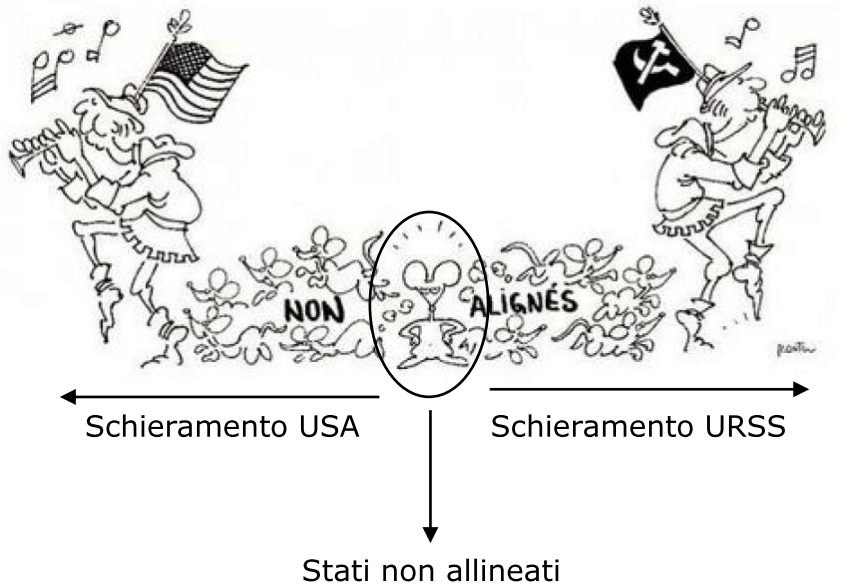
\includegraphics[width=.6\textwidth]{media/bipolarismo.png}
}

La politica di contenimento degli Stati Uniti era mirata a limitare l'espansione sovietica,
intervenendo soprattutto in Asia, America Latina e Medio Oriente.

La tensione tra i due blocchi si manifestava attraverso alleanze militari e aiuti economici,
esercitando un'influenza politica e militare in zone strategiche a livello globale.

\hypertarget{brettonwoods}{\subsubsection{Accordi di Bretton Woods}}
Gli accordi di Bretton Woods ridefinirono l'economia globale dopo la Seconda guerra mondiale.\\
Nel 1944, giudati da Stati Uniti e Gran Bretagna, le principali potenze vittoriose scelsero di
abbandonare il protezionismo\footnote{politica economica che limita le importazioni mediante
dazi e restrizioni per proteggere le industrie nazionali.} a favore di un sistema di commercio
espanso e regole economiche internazionali, per prevenire crisi finanziarie simili a quella del
1929. \vspace*{1.5cm}
\pagebreak

Il valore delle monete fu ancorato al dollaro americano, garantito in oro, permettendo una
gestione economica controllata nei diversi paesi. Questa decisione portò alla creazione di
tre istituzioni fondamentali:
\begin{itemize}
    \item Fondo Monetario Internazionale (FMI);
    \item Banca Internazionale per la Ricostruzione e lo Sviluppo (BIRS);
    \item Accordo generale sulle tariffe doganali e sul commercio (GATT), predecessore
        dell'Organizzazione Mondiale del Commercio (WTO).
\end{itemize}

Queste istituzioni promossero la stabilità monetaria, il finanziamento per la ricostruzione e
lo sviluppo e il commercio multilaterale. I risultati furono significativi:
quasi tre decenni di crescita economica continua, periodo conosciuto come 
\underline{``Età dell'oro del capitalismo regolamentato"}.

\paragraph{Accordi di Bretton Woods: Riassunto} \phantom{}

Gli accordi erano basati sulle conseguenze della crisi del 1929 ed erano mirati ad evitare che
nascessero tensioni post-sanzioni belliche globali. Gli obiettivi principali erano:
\begin{itemize}
    \item Espandere il commercio internazionale;
    \item Accordare regole vincolanti per le espansioni del commercio;
    \item Adeguare i cambi delle valute con un sistema stabile.
\end{itemize}

Le dirette conseguenze agli accordi di Bretton Woods furono la nascita dei seguenti corpi economici:
\begin{itemize}
    \item Fondo Monetario Internazionale (FMI);
    \item Banca Internazionale per la Ricostruzione e lo Sviluppo (BIRS);
    \item Accordo generale sulle tariffe doganali e sul commercio (GATT, diventato WTO nel 1995)
\end{itemize}

\subsubsection{I ``Trenta gloriosi"}
Il termine "Trenta gloriosi" si riferisce al periodo di notevole crescita economica in Europa
dal 1950 al 1973.

Quest'era è caratterizzata dalla ricostruzione post-bellica, dall'espansione dell'economia di
mercato e dall'intervento dello Stato sociale, portando a una ridistribuzione più equa della
ricchetta e a una significativa riduzione della disoccupazione. 

Le sue principali caratteristiche furono:
\begin{itemize}
    \item Stato sociale estero (Welfare State):\\ Stato che si impegna a garantire il benessere dei cittadini,
    investendo significamente in salute pubblica e altri servizi sociali;
    \item Aumento dei posti di lavoro $\Longleftrightarrow$ Diminuzione della disoccupazione;

    \item Forte crescita economica.
\end{itemize}

Le ragioni e le cause del boom economico furono:
\begin{itemize}
    \item Stabilità del nuovo sistema economico;
    \item Nuovi accordi sul commercio mondiali (\hyperlink{brettonwoods}{\color{blue}\underline{Bretton Woods}});
    \item \hyperlink{marshall}{\color{blue}\underline{Piano Marshall}};
    \item Progressi nella ricerca scientifica ed evoluzione tecnologica;
    \item Boom di natalità demografica;
    \item Imposizione e diffusione del modello Fordista:\\
        Assegnazione di singole parti di produzione di un grande progetto composto da molteplici parti;
    \item Disponibilità di fonti energetiche a basso prezzo (petrolio e gas naturale).
\end{itemize}

\pagebreak

\subsection{L'eta della Crisi (1973 - 1991)}
\subsubsection{Modello socialdemocratico}
Il modello socialdemocratico rappresenta un approccio politico ed economico che fonde aspetti
del capitalismo con un robusto intervento dello Stato, mirato a garantire il benessere sociale.
Questo modello si basa su uno Stato sociale (Welfare State).

Le sue principali caratteristiche sono:
\begin{itemize}
    \item Sostegno attivo delle istituzioni europeiste e internazionali (es. ONU);
    \item Integrazione dei sindacati e organizzazioni dei lavoratori nei processi decisionali
        economici e sociali, favorendo la negoziazione collettiva per migliorare le condizioni
        lavorative;
    \item Diritti civili, libertà individuale e partecipazione democratica che garantisce un
        sistema politico aperto e inclusvo;
    \item Economia di mercato equilibrata tra un settore privato dinamico e un aiuto significativo
        dello Stato.\\ L'equità fra sistema statale e privato è chiamato Statalismo.
\end{itemize}

\subsubsection{Crisi petrolifera del 1973}
Le più grandi crisi del petrolio si verificarono nel 1973 e nel 1979.

Il settore delle compagnie petrolifere nel dopoguerra venne influenzato da svariati fattori
politici: gli Stati Uniti decisero di tagliare la produzione petrolifera per dare priorità
alla conservazione delle risorse.\\
Questa decisione portò a un importante incremento di produzione nel Medio Oriente, Africa
Settentrionale e Unione Sovietica.

Come prima conseguenza, nel 1973 l'\underline{OPEC (Organizzazione dei Paesi Esportatori di Petrolio)}
incrementò i prezzi del petrolio. 

L'inflazione e la scarsità petrolifera influenzò la sua fornitura mondiale e portò allo
sviluppo di nuovi metodi di approvvigionamento energetico e allo studio di nuovi metodi per
generare energia a basse emissioni.

Le conseguenze della crisi petrolifera furono:
\begin{itemize}
    \item Coscienza di una necessità del risparmio energetico:
    \begin{itemize}
        \item Sviluppo di nuove tecnologie;
        \item Studio per un'efficienza energetica maggiore;
    \end{itemize}
    \item Dipendenza dal petrolio ridotta;
    \item Potenziamento di fonti energetiche alternative (carbone, gas naturale, nucleare, ...);
    \item Sostituzione di materiali ad alto costo energetico (alluminio, acciaio) con materiali
        più ecosostenibili (plastiche, leghe);
    \item Incentivi per il riciclaggio e per le attività a basso consumo energetico.
\end{itemize}

\subsubsection{L'ondata liberista in occidente}
\paragraph*{Fine del modello socialdemocratico (ca. 1975)} \phantom{}

Gli anni '70 furono segnati dalle crisi petrolifere che causarono inflazione e stagnazione
economica (stagflazione) nei paesi occidentali. Ciò mise in difficoltà i governi
socialdemocratici che faticavano a mantenere il Welfare State senza aumentare il debito pubblico.

Il modello socialdemocratico fu criticato per la sua inefficienza economica e la pesante
burocrazia. Parallelamente nacque una corrente di pensiero che promuoveva il mercato libero e
la riduzione del ruolo dello Stato nell'economia.

\paragraph*{Crisi del Sistema Comunista} \phantom{}

Molti paesi comunisti soffrivano di bassa produttività, scarsa qualità dei beni, innovazione
limitata e inefficiente ripartizione delle risorse.

Leader come Gorbačëv tentarono di riformare il sistema sovietico con politiche come la 
Perestrojka e la Glasnost, ma queste riforme non riuscirono a prevenire il collasso politico.

Il sistema comunista in Europa orientale crollò tra la fine degli anni '80 e l'inizio degli
anni '90, iniziando con la cadutoa del Muro di Berlino nel 1989 e terminando con la fine
della Guerra fredda e la dissoluzione dell'Unione Sovietica nel 1991.

\paragraph*{Ondata liberista} \phantom{}

La fine degli anni '70 e '80 videro l'ascesa di leader che promisero politiche di
deregolamentazione, privatizzazione e tagli fiscali.

L'ondata liberista coincise con un'accelerata globalizzazione, che favorì la libera circolazione
di capitali, beni e servizi a livello globale, aumentando la competizione e l'efficienza 
economica.

Sebbene l'ondata liberista abbia portato a significativi tassi di crescita economica in molti 
paesi, fu criticata per aver aumentato la disuguaglianza di reddito e per aver ridotto la rete
di sicurezza sociale, specialmente nei paesi precedentemente socialdemocratici.
\pagebreak

\section{La globalizzazione tra XX e XXI secolo}
\subsection{La geografia del comportamento}
Dal documento: \href{https://github.com/matteofrongillo/passerella/blob/main/Geografia/media/Pass_03a_GlobalizzazioneXX-XXI-A_22-23.pdf?raw=true}{La geografia del comportamento}

\subsubsection{Globalizzazione e cambiamenti geopolitici}
Dopo la Seconda Guerra Mondiale, il mondo è passato da un equilibrio bipolare durante la Guerra
fredda alla supremazia unipolare degli Stati Uniti seguendo il crollo dell'URSS.

Questo cambio ha facilitato accordi economici transcontinentali come il NAFTA (North American Free Trade Agreemen)
e l'espansione dell'APEC (Gruppo di cooperazione economica Asia-Pacifico), che hanno promosso la
liberalizzazione del commercio e incrementato la cooperazione economica tra i continenti.

\subsubsection{Impatti sociali ed economici}
Nei decenni '80 e '90, l'indebitamento crescente nei paesi in via di sviluppo, aggravato da
politiche monetarie restrittive come quelle degli Stati Uniti, ha portato a profonde crisi
economiche.

Le condizionalità imposte dal FMI (Fondo Monetario Internazionale), come le riforme strutturali
e le politiche di austerità, hanno spesso esacerbato le difficoltà economiche nei paesi in via
di sviluppo, peggiorando la miseria e l'instabilità sociale.

\subsubsection{Evoluzione tecnologica e impatto economico}
L'epoca post-bellica fino gli anni '70 è stata dominata dal modello fordista-keynesiano, che ha
favorito una produzione di massa basata su economie di scala. Questo modello è stato
gradualmente sostituito dal toyotismo e dalla produzione snella, le quali hanno introdotto una
maggiore flessibilità ed efficienza nella produzione.

La seconda metà del XX secolo ha visto un forte impulso verso la finanziarizzazione 
dell'economia, con la rivoluzione informatica che ha trasformato le economie globali, facilitando
una maggiore transnazionalizzazione e diminuendo il controllo statale.

\begin{figure}[h!]
    \centering
    \begin{tabular}{|l|l|}
        \hline 
        \textbf{Fordismo} & \textbf{Post-fordismo} \\
        \hline 
        \begin{tabular}{@{}l@{}}
            - Modello di organizzazione industriale \\ 
            \; tipico nel Novecento
        \end{tabular} & 
            - Modello organizzativo post-industriale \\
        \hline 
        \begin{tabular}{@{}l@{}}
            - Predominantemente nel Settentrione \\
            \; europeo e in America nel dopoguerra
        \end{tabular} & 
        \begin{tabular}{@{}l@{}}
            - Emergenza a partire dagli anni '70 e ' 80 \\
            \; del Novecento
        \end{tabular} \\
        \hline 
        \begin{tabular}{@{}l@{}}
            - Produzione in serie di grandi \\
            \; stabilimenti
        \end{tabular} & 
            - Flessibilità produttiva \\
        \hline 
        \begin{tabular}{@{}l@{}}
            - Produzione basata sulla \\
            \; standardizzazione e sull'efficienza
        \end{tabular} & 
        \begin{tabular}{@{}l@{}}
            - Produzione differenziata, mirata alla \\
            \; personalizzazione
        \end{tabular} \\
        \hline 
        \begin{tabular}{@{}l@{}}
            - Economia basata sull'espansione di \\
            \; mercati potenzialmente infiniti
        \end{tabular} & 
        \begin{tabular}{@{}l@{}}
            - Produzione di piccoli lotti, spesso in \\
            \; base alla domanda
        \end{tabular} \\
        \hline 
        \begin{tabular}{@{}l@{}}
            - Uso intensivo della forza lavoro \\
            \; umana
        \end{tabular} & 
        \begin{tabular}{@{}l@{}}
            - Maggiore uso di tecnologie e \\
            \; automatismi
        \end{tabular} \\
        \hline 
        \begin{tabular}{@{}l@{}}
            - Stabilimenti come quelli della Ford \\
            \; negli Stati Uniti
        \end{tabular} & 
        \begin{tabular}{@{}l@{}}
            - Decentrare la produzione spostandola \\
            \; vicino ai mercati target
        \end{tabular} \\
        \hline 
        \begin{tabular}{@{}l@{}}
            - Innovazione focalizzata su processi e \\
            \; tecnologia che ottimizzano la \\
            \; produzione in serie \\
            - Vertice del modello con le grandi
        \end{tabular} & 
        \begin{tabular}{@{}l@{}}
            - Innovazione orientata alla \\
            \; diversificazione e all'adattamento rapido \\
            - Emergenza di nuovi poli produttivi \\
            \; flessibili e decentrati
        \end{tabular} \\
        \hline 
        & 
        \begin{tabular}{@{}l@{}}
            - Maggiore interconnessione con \\
            \; l'economia globale e con le reti di \\
            \; informazione \\
            - Importanza crescente delle società \\
            \; transnazionali e delle multinazionali
        \end{tabular} \\
        \hline
        \begin{tabular}{@{}l@{}}
            - Catena di montaggio (prod. in serie)
        \end{tabular} & 
            - Flessibilità, just-in-time \\
        \hline 
        \begin{tabular}{@{}l@{}}
            - Domanda in funzione all'offerta
        \end{tabular} & 
            - Offerta in funzione della domanda \\
        \hline 
        \begin{tabular}{@{}l@{}}
            - Territorializzazione
        \end{tabular} & 
            - Delocalizzazione \\
        \hline 
        \begin{tabular}{@{}l@{}}
            - Mercati specifici "nazionali", seppur \\
            \; comunicanti
        \end{tabular} & 
        \begin{tabular}{@{}l@{}}
            - Mercati "transnazionali" \\
            \; (Stati come ostacolo)
        \end{tabular} \\
        \hline
    \end{tabular}
\end{figure}

\subsubsection{Rivoluzioni digitali}
Gli anni '80 hanno visto una saturazione nei mercati di beni di consumo durevoli nei paesi
sviluppati e una riduzione nella domanda di materie prime tradizionali a favore di nuovi
materiali tecnologici.

Il cambio di secolo ha portato con sé una seconda rivoluzione digitale e una crisi delle
politiche neoliberiste, segnando una nuova era di
``\underline{capitalismo della sorveglianza e informazionale}", con significative implicazioni per
la privacy, la sicurezza e il cambiamento nei rapporti di potere globale, con una tensione
crescente tra Stati Uniti e Cina.

\subsubsection{Riassunto grafico: La geografia del comportamento}
\figbox{
    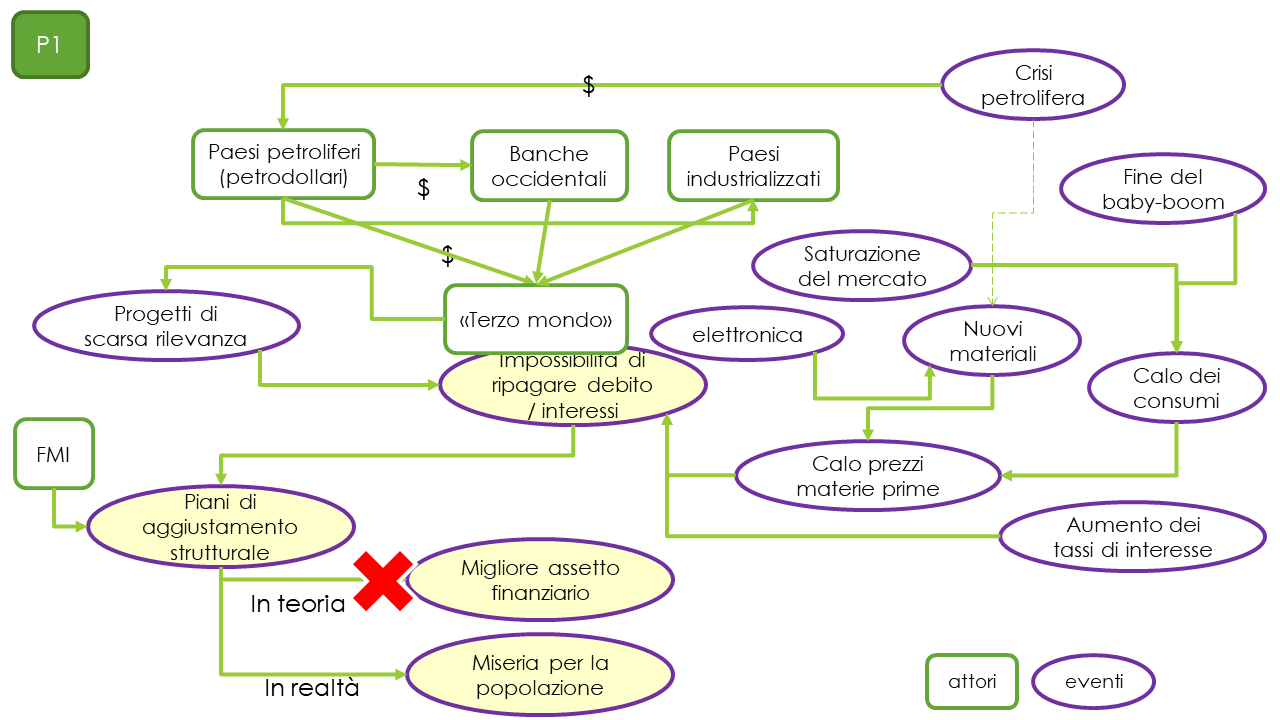
\includegraphics[width=1\textwidth]{media/SchemaP1.png}
}
\pagebreak

\subsection{Nuovi attori e nuove visioni per la scena internazionale }
Dal documento: \href{https://github.com/matteofrongillo/passerella/blob/main/Geografia/media/Pass_03b_GlobalizzazioneXX-XXI-B_22-23.pdf?raw=true}{Nuovi attori e nuove visioni per la scena internazionale}

\subsubsection{Ascesa della Cina come superpotenza}
L'apertura diplomatica tra Stati Uniti e Cina, nel 1973, fu vista come una mossa che permise
alla Cina di emergere come una superpotenza economica e politca, in grado di sfidare la
supremazia americana e partecipare attivamente alla globalizzazione sotto l'egida degli Stati
Uniti.

\subsubsection{Paesi di nuova industrializzazione (NIC)}
Durante la fine degli anni '80 e l'inizio degli anni '90, alcuni paesi in Asia sudorientale,
Africa australe e America Latina trasformarono le loro economie per adattarsi e partecipare ai
grandi circuiti finanziari e commerciali globali.

Accanto a questi paesi emergenti, vi furono paesi gravemente indebitati e paesi poveri con
un'industrializzazione precaria e specializzati in poche materie prime. Queste nazioni
riscontrarono difficoltà crescenti nel contesto globalizzato, evidenziando disparità nella
distribuzione dei benefici della globalizzazione.

\subsubsection{Trasizione dei paesi socialisti}
Sempre nel periodo '80-'90, i paesi socialisti, compresi l'Unione Sovietica e gli stati
dell'Europa centrale, lottarono per adattarsi al nuovo contesto economico globalizzato.
Questo portò al crollo dell'URSS e alla dissoluzione del blocco socialista.

Contrariamente ad altri paesi, la Cina mantenne il suo modello socialista, ma si aprì con
prudenza alla globalizazione, cercando di integrarsi senza rinunciare al controllo statale.

L'integrazione di nuovi attori economici e la trasformazione dei paesi socialisti
ristrutturarono significamente il panorama geopolitico globale.

\subsection{La società polindustriale}
Dal documento: \href{https://github.com/matteofrongillo/passerella/blob/main/Geografia/media/Pass_03b_Sabbatucci_Adreatta_Morin_Aime.pdf?raw=true}{La società polindustriale}

\subsubsection{Testo A: Alla ricerca dell'ordine mondiale - \textit{Andreatta}}
Il biennio tra la caduta del Muro di Berlino e la dissoluzione dell'Unione Sovietica vide
cambiamenti politici e strategici globali di portata storica.

La speranza di un nuovo ordine internazionale più pacifico e cooperativo, fondato su una
co-dominazione USA-URSS, non si realizzò. Le liberalizzazioni nei paesi comunisti innescarono
il crollo dell'URSS.

La fine dell'URSS lasciò un vuoto politico e ideologico significativo, che non fu adeguatamente
colmato dalla Russia postcomunista, portando all'emergere di nuovi nazionalismi e movimenti
politici.

\subsubsection{Testo B: I due principali scenari per il futuro formulati negli anni Novanta - \textit{Morin}}
La dissoluzione dell'equilibrio bipolare facilitò la manifestazione di conflitti localizzati e
l'ascesa di nuove sfide globali, tra cui le divisioni economiche tra Nord ricco e Sud povero, e
le tensioni culturali tra l'Occidente e il mondo islamico.

In un mondo privo di un ordine internazionale chiaro, mancò una leadership globale efficace,
rendendo il panorama internazionale più incerto e trasformando il sistema internazionale in un
terreno di conflitto e transizione inquietante.

\subsubsection{Testo C: Scontri e incontri di culture - \textit{Aime}}
Il contesto storico post Guerra Fredda mise in evidenza come i rapidi cambiamenti avvenuti alla
fine del XX secolo avessero plasmato le dinamiche internazionali, conducendo a una fase di
incertezza e transizione globale.

La crisi di leadership globale evidenziò l'assenza di una direzione chiara, con la Russia
incapace di sostituire l'URSS e gli Stati Uniti e altre potenze emergenti incapaci di gestire da
soli l'ordine mondiale.

\subsubsection{Testo A, B, C in breve}
Nel biennio 1989 (caduta del Muro di Berlino) e il 1991 (dissoluzione dell'URSS), gli
equilibri politici e strategici del pianeta subirono uno sconvolgimento di portata
paragonabile a quelli delle due Guerre mondiali.

Molti speravano che la fine della Guerra fredda portasse un nuovo ordine internazionale più
pacifico e liberale, basato su una co-dominazione tra USA e URSS. Tuttavia, le liberalizzazioni
nei paesi comunisti contribuirono al crollo dell'Unione Sovietica.

La scomparsa dell'URSS creò un vuoto politico e ideologico significativo che la Russia
postcomunista non fu in grado di colmare. Questo portò all'appirizione di nazionalismi e
tendenze politiche precedentemente sopite.

L'assenza di un equilibrio bipolare vide aumentare il numero di conflitti locali e della
creazione di contrapposizioni globali, come la suddivisione tra Nord ricco e Sud povero o
le tensioni culturali tra l'Occidente e il mondo islamico.

In un mondo privo di ordine internazionale venne a mancare una leadership globale efficace,
entrando così in una fase di transizione inqueta senza un ordine internazionale chiaramente
delineato. L'assenza di una leadership rese il panorama mondiale incerto.
\vspace*{.5cm}

\begin{center}
    \begin{tikzpicture}[
        level 2/.style = {sibling distance = 5cm}
    ]
    \node {\Ovalbox{Equilibrio conflitturale}}
        child {
            node {\ovalbox{
                    \begin{minipage}{.10\textwidth}
                        \centering Biennio '89 - '91
                    \end{minipage}
                    }
                }
            child {
                node {\ovalbox{
                        \begin{minipage}{.215\textwidth}
                            \centering Speranza:\\ 
                            Co-dominio tra USA-URSS più pacifico
                        \end{minipage}
                    }
                }
            }
            child {
                node {\ovalbox{
                        \begin{minipage}{.18\textwidth}
                            \centering Realtà:\\ 
                            Dissoluzione URSS
                        \end{minipage}
                    }
                }
                child {
                    node {\ovalbox{
                        \begin{minipage}{.27\textwidth}
                            \centering Conflitti locali, disequilibrio\\
                            e contrapposizioni globali
                        \end{minipage}
                        }
                    }
                }
            }
        };
    \end{tikzpicture}
\end{center}
\phantom{}

\subsubsection{Approfondimento sulla società polindustriale}

\paragraph{La fine della storia - \textit{Fukuyama}}
\begin{quote}
    Fukuyama vede la storia come un processo di continua 
    modernizzazione e sviluppo con un senso ben preciso. L’uomo 
    tenderebbe perciò alla forma di civiltà più elevata, e ciò trova 
    conferma nella destinazione perseguita dai flussi migratori: paesi 
    più ricchi e più sicuri. Questi ultimi, non casualmente, sono tutti 
    caratterizzati da un modello politico democratico, il che porta 
    l’autore a sostenere che l’uomo voglia aderirvi quasi per natura e 
    che, non disponendo di un’evoluzione ulteriore, la storia sia quindi 
    giunta al capolinea. -- (\textit{4F 2019-20, Gruppo 5})
\end{quote} \phantom{}

In altre parole:

Il modello caratterizzato dalla democrazia e dal libero mercato, che alla fine della Guerra
fredda si era imposto, poteva venire considerato il “punto di arrivo” di questo processo.

La tesi è stata elaborata all’inizio degli anni ’90 e che da allora gli avvenimenti hanno in
parte sconfessato o relativizzato quella visione, come l’autore spiega nell’intervista. 

\paragraph{Lo scontro delle civiltà - \textit{Huntington}} \phantom{}

Nel libro di Huntington Lo scontro delle civiltà si delinea una visione del mondo decisamente
originale che si pone in netto contrasto soprattutto con La fine della storia e l'ultimo uomo
di Francis Fukuyama. Se infatti nell'opera di Fukuyama veniva tratteggiata una vera e propria 
"fine della storia" con l'avvento della globalizzazione guidata dalle liberaldemocrazie 
occidentali, secondo Huntington, al contrario, la fine della guerra fredda, non solo non avrebbe
portato all'affermarsi di un modello unico, ma anzi avrebbe liberato le diverse civiltà dal
giogo del bipolarismo politico ed ideologico U.S.A. - U.R.S.S., lasciandole ben più libere di
svilupparsi autonomamente con modi e tempi differenti tra loro.

Tale situazione, secondo Huntington, non sarebbe tuttavia caratterizzata da una pacifica
convivenza […]. L'osservazione di Huntington è quindi proprio che "gli equilibri di potere tra
le diverse civiltà stanno mutando" mentre "l'influenza relativa dell'occidente è in calo".
Le diverse civiltà […] stanno infatti riorientandosi sia su basi ideologiche (ed è questo il
caso del comunismo di mercato che caratterizza quella Sinica) sia, soprattutto, su basi 
religiose (come succede per quella Islamica). L'idea stessa di una civiltà che si afferma sulle
altre come universale è […] del tutto sbagliata e frutto di una visione del mondo schematica e 
ancora legata ai meccanismi della Guerra fredda.

\subsection{BRICS}
Dal documento: \href{https://github.com/matteofrongillo/passerella/blob/main/Geografia/media/Internazionale-BRICS-entrambi.pdf?raw=true}
{Addio ai Bric (2015) / Il vertice dei paesi emergenti in Brasile non fa scalpore (2019)}









\end{document}
